\begin{pages}
    \begin{Rightside}
    \selectlanguage{greek}
        \beginnumbering
        \pstart[
        			\chapter{Ἡ γυνὴ καὶ ὁ δράκων}
        			\markboth{The Woman and the Dragon}
				]
		\renewcommand{\LettrineFontHook}{\PHtitl}
		\lettrine[lines=3]{Κ}{αὶ} σημεῖον μέγα ὤφθη ἐν τῷ οὐρανῷ, γυνὴ περιβεβλημένη τὸν ἥλιον, καὶ ἡ σελήνη ὑποκάτω τῶν ποδῶν αὐτῆς, καὶ ἐπὶ τῆς κεφαλῆς αὐτῆς στέφανος ἀστέρων δώδεκα, καὶ ἐν γαστρὶ ἔχουσα, καὶ κράζει ὠδίνουσα καὶ βασανιζομένη τεκεῖν. 
		\pend
		\pstart
		καὶ ὤφθη ἄλλο σημεῖον ἐν τῷ οὐρανῷ, καὶ ἰδοὺ δράκων πυρρός μέγας, ἔχων κεφαλὰς ἑπτὰ καὶ κέρατα δέκα καὶ ἐπὶ τὰς κεφαλὰς αὐτοῦ ἑπτὰ διαδήματα, καὶ ἡ οὐρὰ αὐτοῦ σύρει τὸ τρίτον τῶν ἀστέρων τοῦ οὐρανοῦ, καὶ ἔβαλεν αὐτοὺς εἰς τὴν γῆν. καὶ ὁ δράκων ἕστηκεν ἐνώπιον τῆς γυναικὸς τῆς μελλούσης τεκεῖν, ἵνα ὅταν τέκῃ τὸ τέκνον αὐτῆς καταφάγῃ. καὶ ἔτεκεν υἱόν, ἄρσεν, ὃς μέλλει ποιμαίνειν πάντα τὰ ἔθνη ἐν ῥάβδῳ σιδηρᾷ· καὶ ἡρπάσθη τὸ τέκνον αὐτῆς πρὸς τὸν Θεὸν καὶ πρὸς τὸν θρόνον αὐτοῦ.
		\pend
		\pstart
		καὶ ἡ γυνὴ ἔφυγεν εἰς τὴν ἔρημον, ὅπου ἔχει ἐκεῖ τόπον ἡτοιμασμένον ἀπὸ τοῦ Θεοῦ, ἵνα ἐκεῖ τρέφωσιν αὐτὴν ἡμέρας χιλίας διακοσίας ἑξήκοντα. Καὶ ἐγένετο πόλεμος ἐν τῷ οὐρανῷ, ὁ Μιχαὴλ καὶ οἱ ἄγγελοι αὐτοῦ τοῦ πολεμῆσαι μετὰ τοῦ δράκοντος. καὶ ὁ δράκων ἐπολέμησεν καὶ οἱ ἄγγελοι αὐτοῦ, καὶ οὐκ ἴσχυσαν, οὐδὲ τόπος εὑρέθη αὐτῶν ἔτι ἐν τῷ οὐρανῷ. 
		\pend
		\pstart
		καὶ ἐβλήθη ὁ δράκων ὁ μέγας, ὁ ὄφις ὁ ἀρχαῖος, ὁ καλούμενος Διάβολος καὶ Ὁ Σατανᾶς, ὁ πλανῶν τὴν οἰκουμένην ὅλην, ἐβλήθη εἰς τὴν γῆν, καὶ οἱ ἄγγελοι αὐτοῦ μετ’ αὐτοῦ ἐβλήθησαν. καὶ ἤκουσα φωνὴν μεγάλην ἐν τῷ οὐρανῷ λέγουσαν Ἄρτι ἐγένετο ἡ σωτηρία καὶ ἡ δύναμις καὶ ἡ βασιλεία τοῦ Θεοῦ ἡμῶν καὶ ἡ ἐξουσία τοῦ 	Χριστοῦ αὐτοῦ, ὅτι ἐβλήθη ὁ κατήγωρ τῶν ἀδελφῶν ἡμῶν, ὁ κατηγορῶν αὐτοὺς ἐνώπιον τοῦ Θεοῦ ἡμῶν ἡμέρας καὶ νυκτός. 
		\pend
		\pstart
		καὶ αὐτοὶ ἐνίκησαν αὐτὸν διὰ τὸ αἷμα τοῦ Ἀρνίου καὶ διὰ τὸν λόγον τῆς μαρτυρίας αὐτῶν, καὶ οὐκ ἠγάπησαν τὴν ψυχὴν αὐτῶν ἄχρι θανάτου. διὰ τοῦτο εὐφραίνεσθε, οὐρανοὶ καὶ οἱ ἐν αὐτοῖς σκηνοῦντες· οὐαὶ τὴν γῆν καὶ τὴν θάλασσαν, ὅτι κατέβη ὁ διάβολος πρὸς ὑμᾶς ἔχων θυμὸν μέγαν, εἰδὼς ὅτι ὀλίγον καιρὸν ἔχει.
		\pend
		\pstart
		Καὶ ὅτε εἶδεν ὁ δράκων ὅτι ἐβλήθη εἰς τὴν γῆν, ἐδίωξεν τὴν γυναῖκα ἥτις ἔτεκεν τὸν ἄρσενα. καὶ ἐδόθησαν τῇ γυναικὶ αἱ δύο πτέρυγες τοῦ ἀετοῦ τοῦ μεγάλου, ἵνα πέτηται εἰς τὴν ἔρημον εἰς τὸν τόπον αὐτῆς, ὅπου τρέφεται ἐκεῖ καιρὸν καὶ καιροὺς καὶ ἥμισυ καιροῦ ἀπὸ προσώπου τοῦ ὄφεως. 
		\pend
		\pstart
		καὶ ἔβαλεν ὁ ὄφις ἐκ τοῦ στόματος αὐτοῦ ὀπίσω τῆς γυναικὸς ὕδωρ ὡς ποταμόν, ἵνα αὐτὴν ποταμοφόρητον ποιήσῃ. καὶ ἐβοήθησεν ἡ γῆ τῇ γυναικί, καὶ ἤνοιξεν ἡ γῆ τὸ στόμα αὐτῆς καὶ κατέπιεν τὸν ποταμὸν ὃν ἔβαλεν ὁ δράκων ἐκ τοῦ στόματος αὐτοῦ. 
		\pend
		\pstart
		καὶ ὠργίσθη ὁ δράκων ἐπὶ τῇ γυναικί, καὶ ἀπῆλθεν ποιῆσαι πόλεμον μετὰ τῶν λοιπῶν τοῦ σπέρματος αὐτῆς, τῶν τηρούντων τὰς ἐντολὰς τοῦ Θεοῦ καὶ ἐχόντων τὴν μαρτυρίαν Ἰησοῦ· καὶ ἐστάθη ἐπὶ τὴν ἄμμον τῆς θαλάσσης.	
		\pend
        \endnumbering
    \end{Rightside}
    \begin{Leftside}
        \beginnumbering
        \pstart[
        			\chapter{The Woman and the Dragon}
				]		
		\renewcommand{\LettrineFontHook}{\Zallmanfamily}
		\lettrine[lines=3]{A}{nd} a great sign appeared in Heaven (and it was a) woman wearing the Sun, and the Moon was beneath her feet and upon her head (was a) crown (made out) of twelve stars. And she was pregnant; and she cried out — because she was in labour — and (she was) tormented (greatly) (because she was about) to give birth. 
		\pend
		\pstart
		And there appeared another sign in Heaven — and look! A great fiery dragon having seven heads and ten horns; and upon his heads (there were) seven crowns, and his tail sweeps (away) a third of the stars of Heaven and threw them into the Earth. And the dragon stood before the woman who was about to give birth so that he might eat her child when she gives birth. And she gave birth to a son who was (about) to shepherd (rule, lead) all (the) peoples (of the Earth) with an iron rod; and her child was snatched away by God and (brought? lead?) to His throne. 
		\pend
		\pstart
		And the woman fled into the wilderness where she had a place (there) prepared (for her) of God so that they might nourish her there for one-thousand two-hundred sixty days. And a war began (was, happened) in Heaven (in which) Michael and his angels fought (with) the dragon — and the dragon, too, fought and his angels (along with him). But they did not prevail, nor was their place to be found in Heaven any longer (when the battle had finished). 
		\pend
		\pstart
		And the great dragon was thrown — (the great dragon), the ancient serpent; the one called Devil and Satan; the deceiver of the entire (inhabited) world. He was thrown into (onto) the Earth and his angels were thrown (along) with him. And I heard a great voice in Heaven saying, “Now has come the deliverance and the power and the kingdom of our God and the authority (power) of His Messiah; for the accuser of our brothers — who accused them before our God day and night — has been cast (into the Earth). 
		\pend
		\pstart
		And they prevailed over him because of the blood of the Lamb and because of the word of His witness — and they did not love their own souls more than death (they weren’t afraid of dying). Therefore rejoice, O Heavens and those dwelling therein. Woe to the Earth and the sea, for the Devil — bearing (with him) a great wrath — has descended (down) towards you, knowing that he has (but) little time (left).”
		\pend
		\pstart
		And when the dragon saw (realised) that he was thrown into (down onto) the Earth, he (began) persecuting the woman who gave birth to the boy. But (and) there were given to the woman the two wings of the great eagle, so that she might fly into the wilderness — into her place — where she is (will be) nourished for a time and times and half a time from the face of the serpent. 
		\pend
		\pstart
		But (and) then the serpent spewed forth (threw) water — like a river — so that she might be made to be carried off (by the river). But (and) the Earth shouted for the (sake of the) woman, and the Earth opened its mouth and swallowed (ate up) the river which the dragon spewed forth (threw) from its mouth. 
		\pend
		\pstart
		And the dragon became angry with (on) the woman and left to wage war against (make war with) the remaining of her offspring — the ones honouring the commandments of God and (the ones which have) the witness of Jesus; and he stood upon the sand of the sea. 
		\pend
        \endnumbering
    \end{Leftside}

\end{pages} 
\Pages

\clearpage
\thispagestyle{empty}
\null\vfill
\settowidth\longest{\huge\itshape […] and when I turned around I saw}
\begin{center}
\parbox{\longest}{%
  \raggedright{\huge\itshape%
    ``And there appeared another sign in Heaven — and look! A great fiery dragon having seven heads and ten horns.'' \par\bigskip
  }
  \raggedleft\Large\MakeUppercase{``The Great Red Dragon and the Woman Clothed with the Sun'' — William Blake, between 1803 – 1805}\par%
}
\vfill\vfill
\clearpage\newpage
\end{center}
\newpage
\thispagestyle{empty}
\begin{center}
	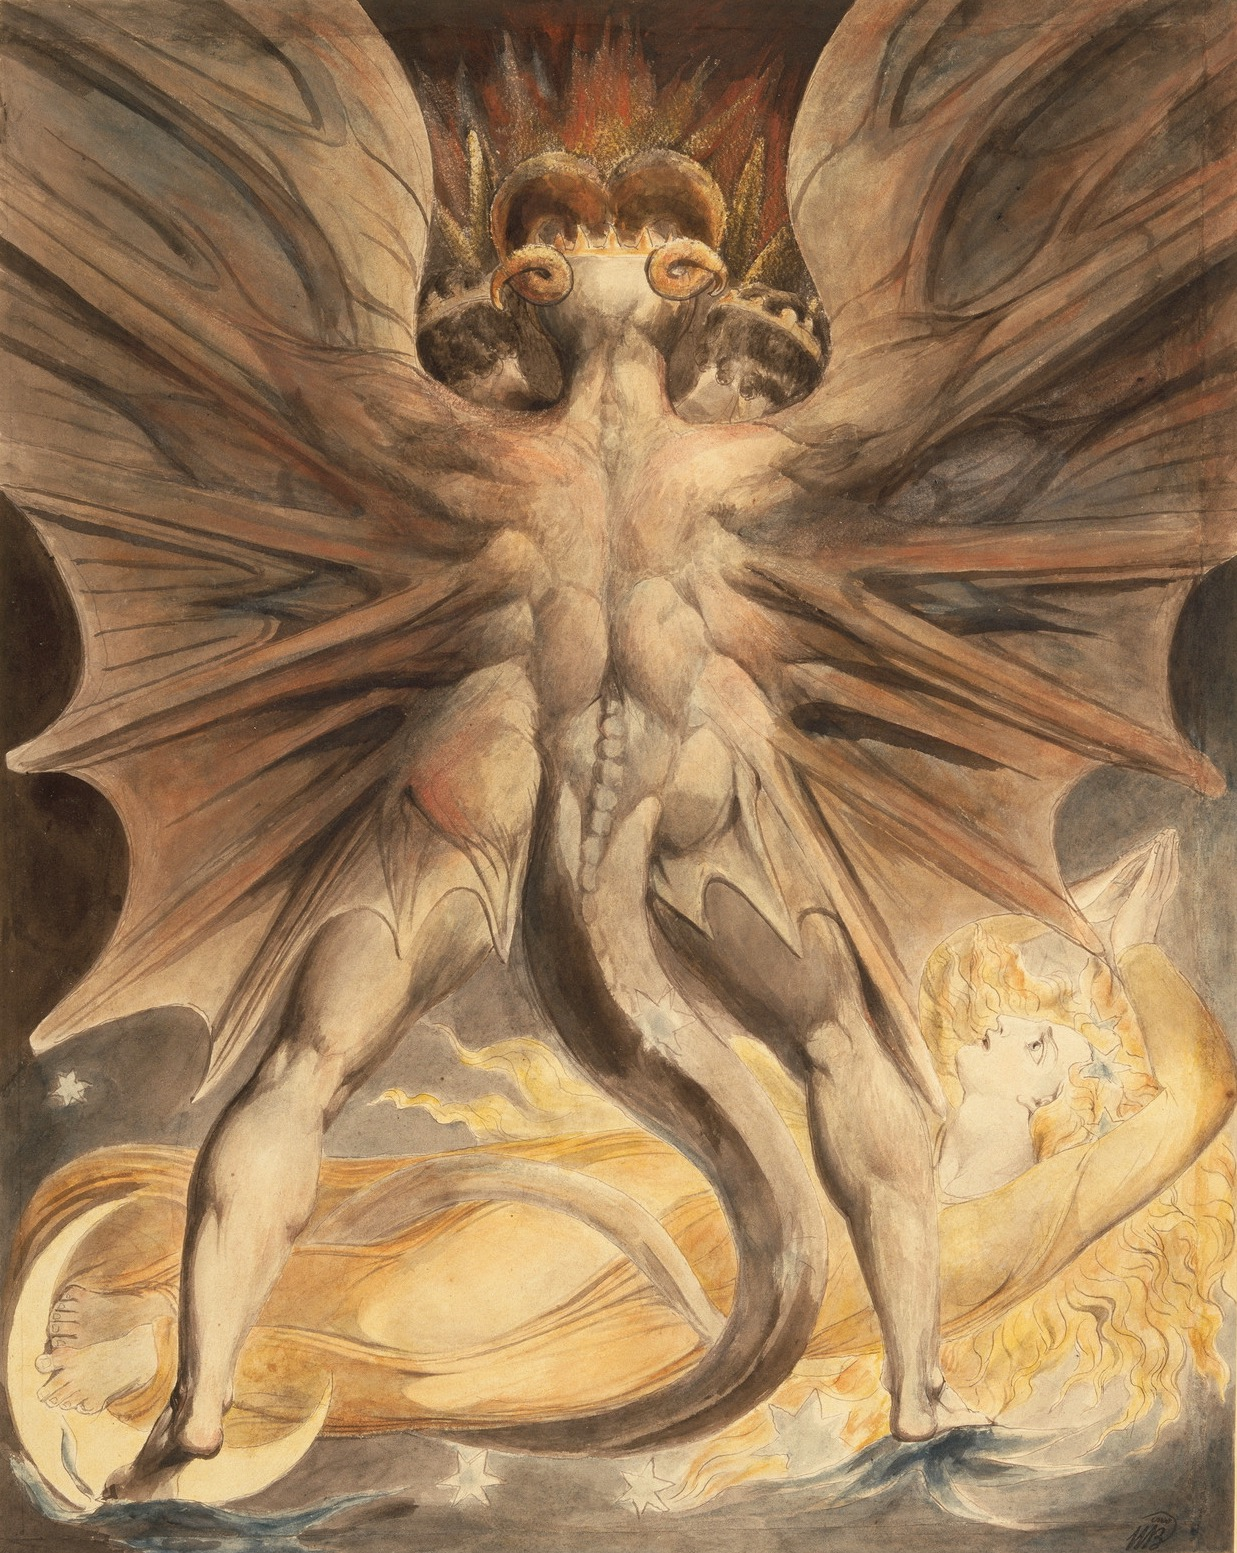
\includegraphics[width=1\textwidth]{images/illustrations/blakedragonwoman}
\end{center}